\chapter{Big-Data Processing and Feature Engineering}
\label{chap:data}

\section{Source validation and typed ingestion}

The raw IEEE-CIS dataset contains four required CSV files totaling \val{1.29~GB}, as shown in Table~\ref{tab:source-files}. This size, combined with the wide schema and the need for repeated joins and aggregations, motivates the use of Spark rather than an ad hoc in-memory workflow. The ingestion stage applies explicit schemas instead of relying on automatic type inference, checks that every required file is present, and records the source inventory so that later results can be traced back to a known input state.

The source validation stage also treats the transaction identifier as a data
quality control rather than merely a join key. Null identifiers and duplicate
identifiers can change the grain of the dataset, create accidental row
multiplication, or make a later prediction impossible to trace to its source.
The pipeline therefore validates identifier presence and uniqueness before
enrichment. It normalises the identity-side naming convention where needed so
that train and test records follow the same join semantics. These checks are
particularly important in an anonymised competition dataset because column
names alone do not provide enough business meaning to detect a broken join.

\begin{table}[H]
\centering
\small
\rowcolors{2}{ReportGray!25}{white}
\caption{Observed source files}
\label{tab:source-files}
\begin{tabularx}{\textwidth}{Xrr}
\toprule
\textbf{File} & \textbf{Bytes} & \textbf{Role}\\
\midrule
\texttt{train\_transaction.csv} & \val{683,351,067} & Labeled transactions\\
\texttt{train\_identity.csv} & \val{26,529,680} & Optional train identity\\
\texttt{test\_transaction.csv} & \val{613,194,934} & Unlabeled transactions\\
\texttt{test\_identity.csv} & \val{25,797,161} & Optional test identity\\
\bottomrule
\end{tabularx}
\end{table}

The source-file table demonstrates both the scale and the two-table structure
of the workload. Transaction files dominate storage and row count, while the
identity files are smaller but provide additional context for only a subset of
transactions. This asymmetry explains why the pipeline treats transactions as
the authoritative grain and preserves unmatched identity information.

\section{Join integrity}

Row authority is preserved through a LEFT JOIN on \texttt{TransactionID}, with the audit shown in Table~\ref{tab:join-audit}. Every transaction row remains present after enrichment: the train join retains all \val{590,540} transactions and the test join retains all \val{506,691} transactions. The large unmatched counts are not treated as join failures because identity data is optional in the competition dataset. Instead, they are preserved as measurable missingness, allowing downstream analysis to distinguish an absent identity record from an invalid transaction key.

The join audit separates three cases that are often conflated in fraud
pipelines. A transaction can have a valid identity match, can be a legitimate
transaction with no identity record, or can reveal a genuine data-integrity
problem such as a duplicated key. Only the third case should be treated as a
join defect. Preserving the first two cases lets the model learn whether the
presence or absence of identity evidence itself is informative, while the
row-difference check ensures that the enrichment stage has not silently
changed the number of transactions under evaluation.

\begin{table}[H]
\centering
\small
\rowcolors{2}{ReportGray!25}{white}
\caption{Transaction--identity join audit}
\label{tab:join-audit}
\begin{tabular}{lrrrr}
\toprule
\textbf{Dataset} & \textbf{Transactions} & \textbf{Identity matches} & \textbf{Unmatched} & \textbf{Row difference}\\
\midrule
Train & \val{590,540} & \val{144,233} & \val{446,307} & \val{0}\\
Test & \val{506,691} & \val{141,907} & \val{364,784} & \val{0}\\
\bottomrule
\end{tabular}
\end{table}

The join audit confirms that enrichment does not alter the transaction grain.
There are \val{144,233} identity matches in train and \val{141,907} in test,
but unmatched transactions remain part of the dataset instead of being
discarded. The zero row difference in both datasets is the key integrity
result: missing identity information is represented as missingness, not as
accidental loss of transactions.

\section{Leakage-controlled transformation order}

The transformation order is designed around a strict information boundary. Aggregate statistics, imputation values, categorical mappings, and any other learned preprocessing state are fitted only on the training partition. The frozen state is then applied forward to validation and holdout data without refitting. Figure~\ref{fig:final-detailed-pipeline} details this sequence. This is important because a random or leakage-prone preprocessing step could allow information from later transactions to influence the model before evaluation, producing metrics that are higher than the model's likely future performance.

\begin{figure}[H]
\centering
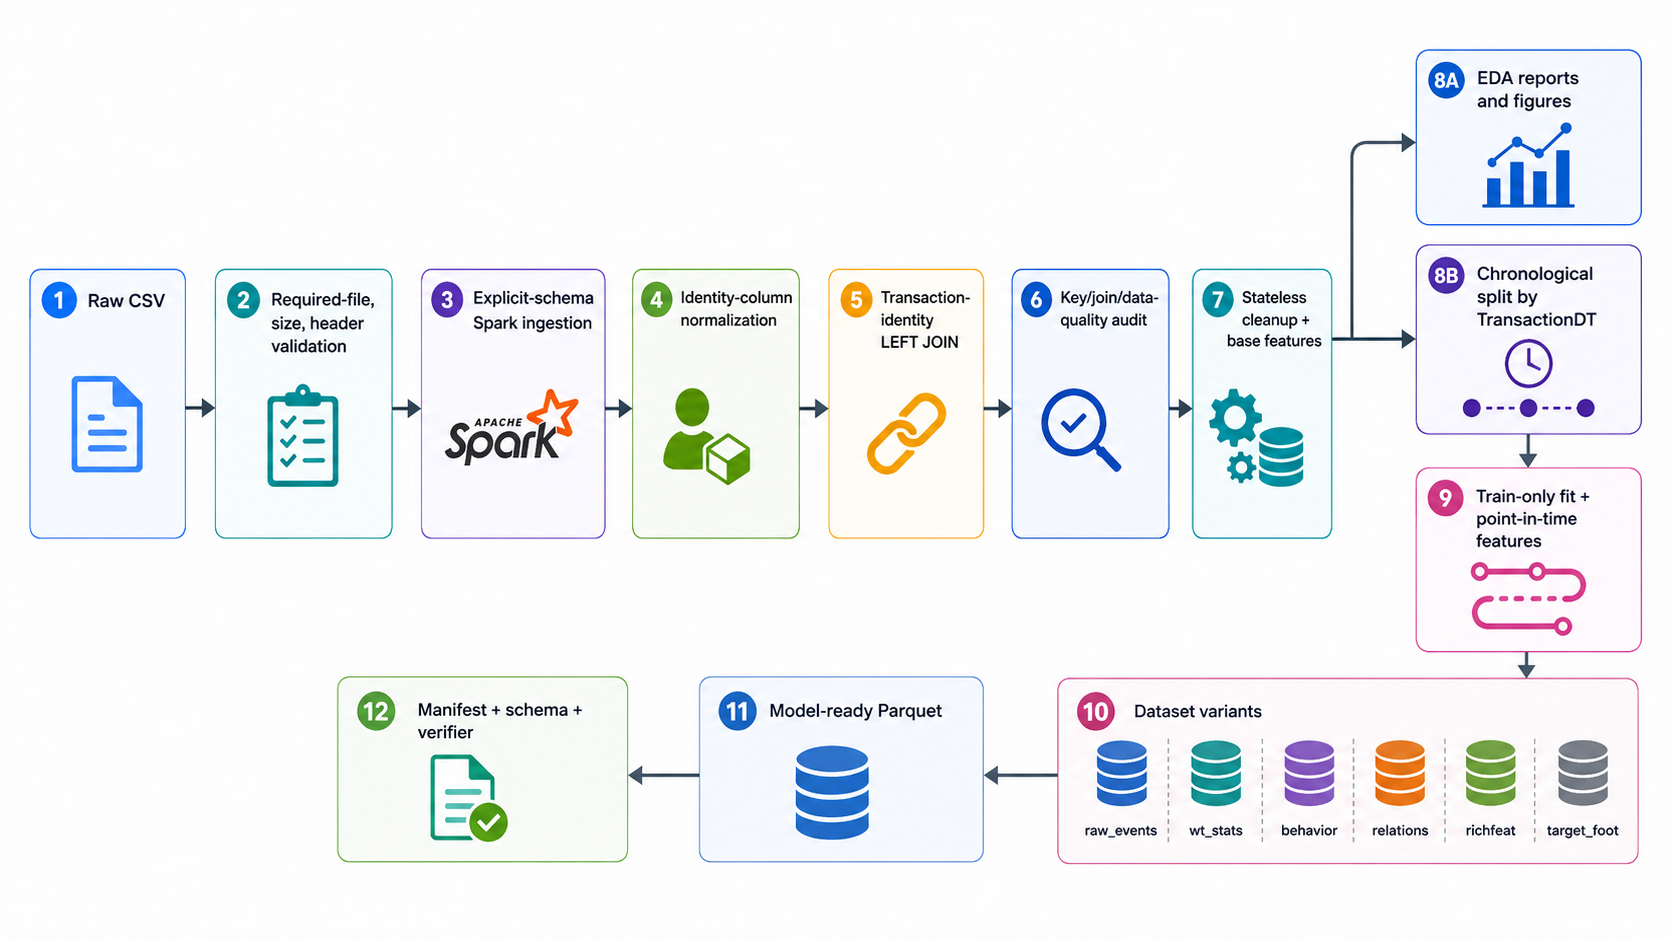
\includegraphics[width=\textwidth,height=0.80\textheight,keepaspectratio]{../../docs/diagrams/final/detailed-data-processing-pipeline.png}
\caption[Detailed data processing pipeline]{Detailed data processing pipeline (AS-BUILT). EDA is a reporting branch; it is not represented as a mandatory transformation of the model-ready data.}
\label{fig:final-detailed-pipeline}
\end{figure}


\section{Chronological split}

Sorting by \texttt{TransactionDT} creates non-overlapping chronological splits, summarized in Table~\ref{tab:chronological-splits}. The training window contains the earliest labelled transactions, the validation window represents a later period used for model and threshold decisions, and the holdout window is reserved for the final evaluation. The fraud rates remain close to the overall rate across the three windows, but the time separation is still essential because fraud mechanisms, merchant behaviour, and missingness patterns can change over time.

\begin{table}[H]
\centering
\small
\rowcolors{2}{ReportGray!25}{white}
\caption{Chronological labeled splits}
\label{tab:chronological-splits}
\begin{tabular}{lrrrr}
\toprule
\textbf{Dataset} & \textbf{Rows} & \textbf{Fraud} & \textbf{Fraud rate} & \textbf{\texttt{TransactionDT} range}\\
\midrule
Train & \val{412,956} & \val{14,522} & \val{3.5166\%} & \val{86,400}--\val{10,432,902}\\
Validation & \val{88,486} & \val{3,036} & \val{3.4310\%} & \val{10,432,915}--\val{13,136,583}\\
Holdout & \val{89,098} & \val{3,105} & \val{3.4849\%} & \val{13,136,627}--\val{15,811,131}\\
\bottomrule
\end{tabular}
\end{table}

The split table shows that the three evaluation windows are separated by
\texttt{TransactionDT} and retain similar fraud rates. Training provides the
historical learning window, validation is used for candidate and threshold
decisions, and holdout represents later unseen data. Similar prevalence makes
the comparison easier to interpret, but it does not remove the possibility of
temporal feature or behaviour shift.

\section{Feature engineering \& class balance}

The canonical \val{68}-feature vector combines several types of evidence rather than depending on one raw column family. It includes transaction time and amount, indicators describing missingness, anonymized behavioural variables such as \texttt{C1--C14} and \texttt{D1--D15}, historical aggregates for repeated entities, and selected categorical attributes. Because fraud is rare, the training data is also represented in original, weighted, and controlled-balanced forms. The distribution in Table~\ref{tab:class-balance} shows why class weighting and sampling must be treated as modelling choices: they can improve the model's attention to fraud, but they also change the precision-recall tradeoff and must be evaluated on the naturally imbalanced validation and holdout windows.

Historical entity features are constructed with a temporal constraint. For an
entity such as a card, email, or device, the feature represents information
available from earlier observations rather than a summary that includes the
current or future label. Examples include prior transaction counts, prior
amount statistics, and the existence of previous activity. Such features can
be highly useful in fraud detection because repeated behaviour and sudden
velocity changes often distinguish risky activity. They are also a major
source of leakage if calculated across the complete dataset before splitting,
which is why the training-only and forward-application rules are central to the
pipeline design.

Missingness is retained as a first-class signal. Numeric variables use values
derived from the training partition for imputation, while categorical values
can be represented through an explicit missing category. This avoids using
validation or holdout distributions to determine preprocessing values and
allows the model to distinguish an observed zero from an unavailable value.
The resulting feature contract records the mappings and order needed by both
training and request-time inference.

\begin{table}[H]
\centering
\small
\rowcolors{2}{ReportGray!25}{white}
\caption{Training and evaluation class distributions}
\label{tab:class-balance}
\begin{tabular}{lrrr}
\toprule
\textbf{Dataset} & \textbf{Legitimate} & \textbf{Fraud} & \textbf{Ratio}\\
\midrule
\texttt{train\_original} & \val{398,434} & \val{14,522} & \val{27.44}\\
\texttt{train\_weighted} & \val{398,434} & \val{14,522} & \val{27.44}\\
\texttt{train\_balanced} & \val{43,872} & \val{14,522} & \val{3.02}\\
\texttt{validation} & \val{85,450} & \val{3,036} & \val{28.15}\\
\texttt{holdout} & \val{85,993} & \val{3,105} & \val{27.70}\\
\bottomrule
\end{tabular}
\end{table}

The class-distribution table explains why the project evaluates weighting and
sampling policies separately. Original and weighted datasets preserve the
natural majority-to-fraud ratio, while the balanced dataset changes the
training distribution. Validation and holdout remain naturally imbalanced, so
the effect of a training policy must be judged by realistic ranking and review
metrics rather than by training balance alone.

\section{Verification result}

The automated verifier passes \val{94} checks with zero failures. This result confirms that the exported data satisfies the expected schema, split, feature-order, and contract checks and can be handed to downstream model training. The status is recorded as:

\begin{lstlisting}
ready_for_downstream_training
\end{lstlisting}
